\chapter{Control Flow Integrity Enforcer}
\label{cha:project}

This chapter focuses on \textit{project name}'s implementation. We will see the
goals and specifics of the project as well as a detailed description of every
key aspect of the development. Lastly, a Proof of Concept is discussed to prove
the functioning and security capabilities of \textit{project name}.

\section{Project Formalization}
\label{sec:project_formalization}

This project aims at providing a secure infrastructure for embedded devices
based on the \textit{RISC-V} ISA. The main goal is to protect the device from
control-flow attacks such as Return-Oriented Programming (ROP) attacks. To do so,
\textit{project name} provides a Control Flow Integrity (CFI) Enforcer which ensures
that the software follows the expected path. Moreover, it provides instrumenting
capabilities to automatize the implementation of any code.

Control Flow Integrity is a security technique that does not allow control transfers
that are not part of the Control Flow Graph (CFG) of the binary.

Another goal of this project is to be as lightweight as possible to meet the performance
requirements of less powerful devices. Thus, great importance is given to optimization
of both space and time consumption.

\textit{project name} makes it possible to run untrusted code in a secure
environment protecting the execution path of the software and ensures that any
attack attempt will be detected by the CFI Enforcer and thus, the device will not
be compromised.

This project makes use of \textit{RISC-V} capabilities like the PMP to implement
secure spaces of memory. It also utilizes state-of-the-art solutions like a Shadow
Stack and a Control Flow Graph to ensure the correctness of the policies.

\section{Project Specifics}
\label{sec:project_specifics}

\begin{wrapfigure}
  {l}{.25\textwidth}
  \centering
  \def\stackalignment{l}\stackunder{ 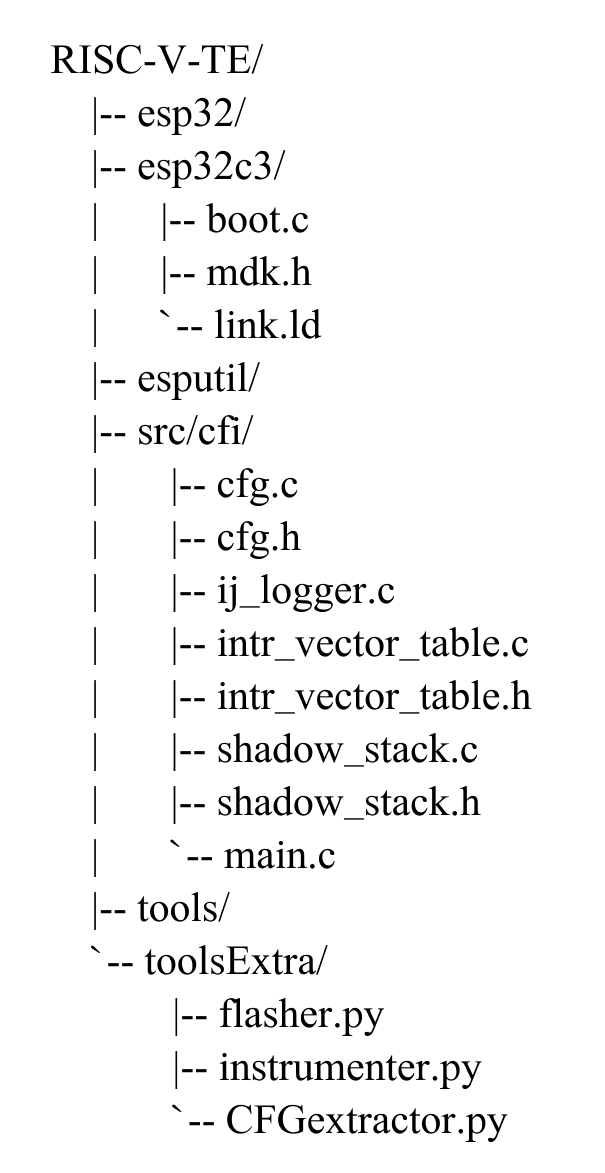
\includegraphics[width=\linewidth]{images/workingtree.png} } %
  {\scriptsize }
  \caption{Working Tree}
  \label{fig:workingtree}
\end{wrapfigure}

The project has been developed on \textit{Espressif's ESP32-C3-DevKitM-1}
\cite{esp32c3} and the basic configuration for bare-metal flashing on such board
is derived by Sergey Lyubka's project \textit{mdk}\cite{mdk}. Lastly, the
\textit{riscv-none-elf}\cite{toolchain} toolchain has been used to cross-compile
the code. However, since the project has been developed following the ideas of
\textit{RISC-V} about hardware abstraction any of these settings can be modified
according to one needs\footnote{Note that if we wish to change the target board,
all vendor-specific files needed to flash the code must replace \textit{Espressif}'s
files}.

Figure \ref{fig:workingtree} depicts the working tree of the project, where:
\begin{itemize}
  \item \textit{esp32} contains the boot configuration and linker script for
    general \textit{Espressif}'s boards;

  \item \textit{esp32c3} contains the boot configuration and linker script for
    the \textit{ESP32-C3};

  \item \textit{esputil} contains \textit{Espressif}'s utils used to manage the board;

  \item \textit{src/cfi/usercode} contains the untrusted code that needs
    protection during execution. The code inside this folder will be the target for
    code instrumentation;

  \item \textit{src/cfi} contains the source files for the Shadow Stack, Control
    Flow Graph, interrupt vector table and machine setup;

  \item \textit{toolsExtra} contains the Python scripts used to instrument, build,
    and flash the code.
\end{itemize}

The scripts inside \textit{toolsExtra} are used to compile, instrument, and run
the code (detailed description in Section \ref{sec:project_instrumentation}). Moreover,
the file \textit{CFGextractor.py} is used to extract the Control Flow Graph of the
code.

Inside \textit{src/cfi} instead, we find the code responsible for managing the machine
mode operations. File \textit{main.c} is responsible for setting up interrupts,
managing privilege modes, and setting up both the PMP (detailed description in
Section \ref{sec:project_pmp}) and the interrupt vector table (detailed
description in Section \ref{sec:project_isr}). File \textit{intr\_vector\_table.c}
is responsible for managing interrupts and exceptions as well as performing controls
on both forward and backward checks (detailed description in Section
\ref{sec:project_controls}). Files \textit{cfg.c} and \textit{shadow\_stack.c}
hold the Control Flow Graph and the Shadow Stack configurations respectively (detailed
description in Sections \ref{sec:project_cfg} and \ref{sec:project_ss}). Lastly,
\textit{ij\_logger.c} is used to retrieve indirect jump addresses thanks to a logger.

\section{Code Instrumentation}
\label{sec:project_instrumentation}

Code instrumentation is the process of modifying software (usually binary or assembly
code) by inserting instructions to perform specific tasks such as a performance
analysis. Instrumentation plays a critical role in this project as it allows to modify
the untrusted code in a simple yet effective way. Moreover, this automatize the process
leading to faster development and lower number of errors. The whole
instrumentation procedure is depicted in Figure \ref{fig:instrumentation}.

\begin{figure}[htbp]
  \centering
  \def\stackalignment{r}\stackunder{ 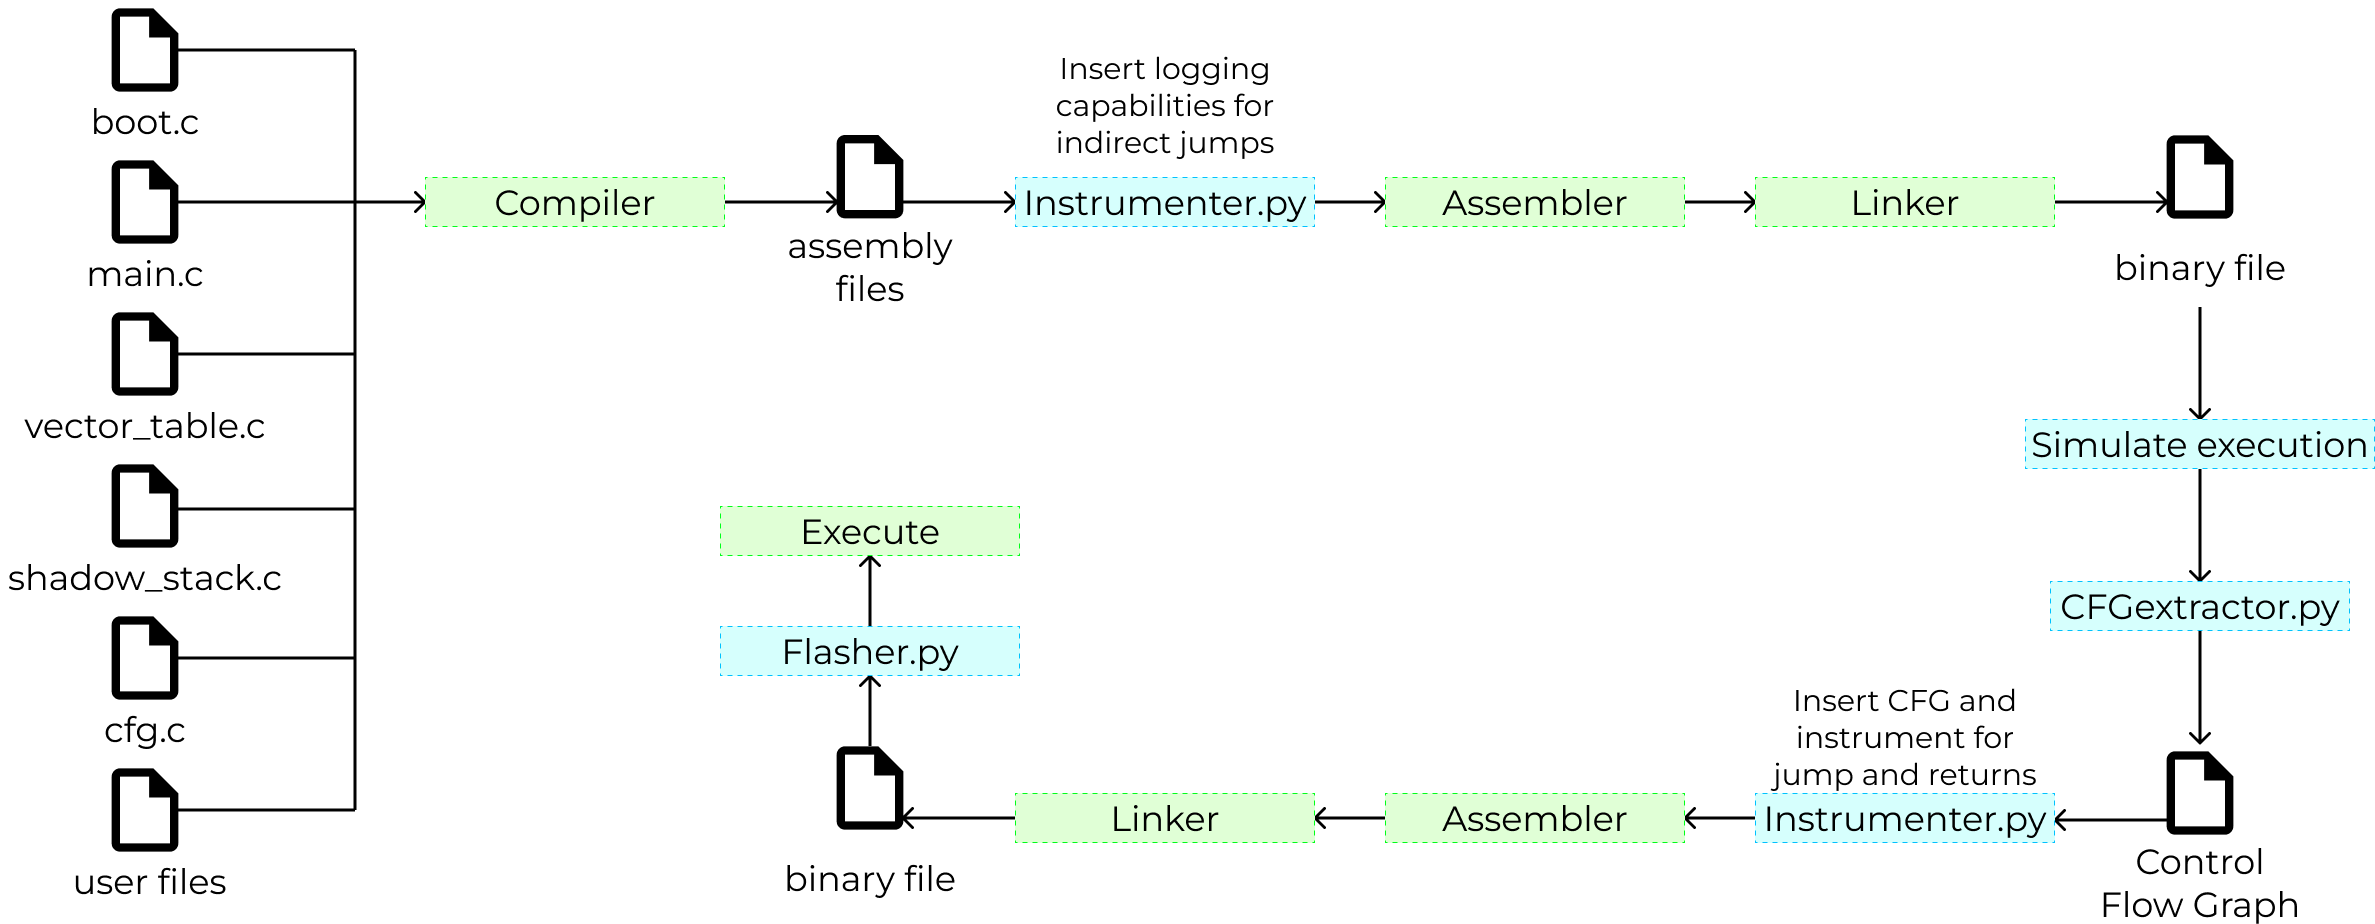
\includegraphics[width=.9\linewidth]{images/instrumentation.png} } %
  {\scriptsize }
  \caption{Flow of the Code Instrumentation Procedure}
  \label{fig:instrumentation}
\end{figure}

The script \textit{flasher.py} can be run with the command \textit{python3
flasher.py [command]}, where \textit{command} can be:
\begin{itemize}[noitemsep]
  \item \textit{build}: for building the source files and producing the binary;

  \item \textit{run}: for building and running the binary on the target device;

  \item \textit{clear}: for clearing output files in the directory;

  \item \textit{secure-build}: for instrumenting and building the source files and
    producing the secure binary;

  \item \textit{secure-run}: for instrumenting, building, and running the secure
    binary on the target device.
\end{itemize}

As we can see the instrumentation only happens with \textit{secure-build} and
\textit{secure-run} commands. Normal building and running commands have been
implemented to make a comparison between an untrusted code and the trusted one.

\subsection{Instrumentation for logging}
\label{subsec:logging}

If we run \textit{flasher.py} with \textit{secure} commands the instrumentation phase
follows the steps described below.

All source files are compiled into assembly files with the toolchain, then the
untrusted user files are passed to \textit{instrumenter.py}. Firstly, the code is
instrumented with logging capabilities to retrieve indirect jump destinations.
This is done by searching indirect jump instruction (\textit{JALR}) with the regex
\textit{$\backslash$b(jalr)$\backslash$b$\backslash$s+($\backslash$w+)} which
retrieves any occurrence of \textit{jalr \{register\}}\footnote{Usually the
compiler uses register \textit{a5} for \textit{JALR} instructions.}.

\begin{wrapfigure}
  {r}{0.25\textwidth}
  \setlength{\intextsep}{0pt}
  \begin{minipage}{0.25\textwidth}
    \begin{lstlisting}[style=Assembly, caption = Logging code block, label={lst:loggingblock}]
addi sp,sp,-40
sw a5,4(sp)
sw a4,8(sp)
sw a2,12(sp)
sw a1,16(sp)
sw a0,20(sp)
sw s0,24(sp)
sw s1,28(sp)
sw s2,32(sp)
sw s3,36(sp)
mv a1,{register}
auipc a0,0
addi a0,a0,38
call print_reg
lw a5,4(sp)
lw a4,8(sp)
lw a2,12(sp)
lw a1,16(sp)
lw a0,20(sp)
lw s0,24(sp)
lw s1,28(sp)
lw s2,32(sp)
lw s3,36(sp)
addi sp,sp,40
jalr {register}
    \end{lstlisting}
  \end{minipage}
\end{wrapfigure}

Once we retrieve the source register for the \textit{JALR} instruction we add
the block of code depicted in Listing \ref{lst:loggingblock} before the jump. This
effectively allows us to save the state of the machine and call the function \textit{print\_reg}
passing the destination address and the program counter of the \textit{JALR} instruction
as arguments. The destination address is simply stored in the source register
while the source address is computed by loading the current program counter with
\textit{auipc a0, 0} and by adding $38$\footnote{Note that $38$ is the distance
in Bytes from the instruction that load the \textit{pc} to the \textit{JALR}
instruction.} to it. The \textit{print\_reg} function, when called, will then
print a string like \textit{Source: 0x40380100 - Destination:0x40380200}.

\subsection{Control Flow Graph Extraction}
\label{subsec:project_cfgextraction}

As soon as the first instrumentation is completed, the assembly files are assembled
and linked to produce the binary. If, during instrumentation, we have found that
there are indirect jumps in the code we perform a ``simulation''\footnote{The
simulation consists in running the code on the target device transparently.} of the
execution to retrieve the logging of the \textit{print\_reg} function.

After that \textit{CFGextractor.py} is called to extract the Control Flow Graph of
the user code. The extraction is divided in two phases:
\begin{itemize}
  \item Dynamic phase: in the dynamic phase we parse the output retrieved from
    the simulation to create source-destination pairs of addresses. Note that in
    this phase addresses are also adjusted by removing the size of the logging block
    from their value. This is done because, during the simulation we injected the
    logging block before each jump, thus increasing the size of the binary. For each
    address we count the number of blocks that appeared before it and we compute
    $\textit{final\_address}= \textit{retrieved\_value}- (\textit{block\_size}* \textit
    {block\_number})$;

  \item Static phase: in the static phase we simply parse the dump file obtained
    with \textit{riscv-none-elf-objdump} searching for \textit{JAL} instructions.
    These direct jump are statically defined so we can retrieve them with the dump
    file. Each time a \textit{JAL} instruction is found the pair source-destination
    is added to the CFG.
\end{itemize}

Once the Control Flow Graph is extracted, all the pairs are ordered in ascending
ordered firstly by source and then by destination. This is because with indirect
jump instructions we could have that more destinations could share the same
source. After that, execution is returned to \textit{instrumenter.py}.

\subsection{Instrumentation for forward and backward edge controls}
\label{subsec:project_instrcontrols}

In this last instrumentation phase we need to add code blocks that allows us to
perform forward and backward edge controls. Such blocks must be added before every
direct jump, indirect jump, and return instruction. To do so, we parse the assembly
files, and, search for the target instructions thanks to the regex functions depicted
in Table \ref{tab:regexes}.

\begin{table}
  \centering
  \begin{tabular}{|c|c|}
    \hline
    \textbf{Regex}                                                                      & \textbf{Use}                            \\
    \hhline{==} \textit{$\backslash$b(call)$\backslash$b$\backslash$s+($\backslash$w+)} & Used to find \textit{JAL} instructions  \\
    \hline
    \textit{$\backslash$b(jalr)$\backslash$b$\backslash$s+($\backslash$w+)}             & Used to find \textit{JALR} instructions \\
    \hline
    \textit{$\backslash$b(jr)$\backslash$b$\backslash$s+($\backslash$w+)}               & Used to find \textit{RET} instructions  \\
    \hline
  \end{tabular}
  \caption{Regex functions used to find target instructions}
  \label{tab:regexes}
\end{table}

Depending on the instruction we find during parsing we do the following:
\begin{itemize}
  \item \textit{JAL} instructions: if we find a direct jump instruction we need to
    add the code depicted in Listing \ref{lst:dirjumpblock} before the target.
    This code loads the address of the target function in register \textit{a7} and
    then performs and \textit{ECALL} instruction (detailed functioning explained
    in \ref{sec:project_isr});

  \item \textit{JALR} instructions: if we find an indirect jump instruction we need
    to add the code depicted in Listing \ref{lst:indirjumpblock} before the target.
    This code copies the address stored in the target register into register
    \textit{a7} and then performs and \textit{ECALL} instruction;

  \item \textit{RET} instructions: if we find a return instruction we need to add
    the code depicted in Listing \ref{lst:retblock} before the target. This code
    copies the return address stored in the return address register into
    register \textit{a7} and then performs and \textit{ECALL} instruction. In Section
    \ref{sec:project_isr} we will see why, in this case, we need to add $1$ to the
    return address.
\end{itemize}

\begin{lstlisting}[style=Assembly, caption = Direct jump code block, label={lst:dirjumpblock}]
la a7, {target_function}
ecall
jal {target_function}
\end{lstlisting}

\begin{lstlisting}[style=Assembly, caption = Indirect jump code block, label={lst:indirjumpblock}]
mv a7, {target_register}
ecall
jalr {target_register}
\end{lstlisting}

\begin{lstlisting}[style=Assembly, caption = Return code block, label={lst:retblock}]
addi a7, {return_address_register}, 1
ecall
addi {return_address_register}, a7, -1
ret {return_address_register}
\end{lstlisting}

In the last step of the instrumentation we inject the previously crafted Control
Flow Graph into the \textit{cfg.c} file.

After this second instrumentation ends, the modified assembly files are assembled
and linked by \textit{flasher.py} to produce the secure binary file. Lastly, if
we used the \textit{secure-run} command, the binary file is flashed on the
target device for execution.

\section{Interrupts Service Routine}
\label{sec:project_isr}

In this section, we will see how the interrupt vector table is implemented and
how interrupts and exceptions are handled in this project. Most importantly we will
see how forward and backward edge controls are enforced.

The interrupt vector table is defined inside \textit{intr\_vector\_table.c}. As already
explained its address is loaded in \textit{main.c} and stored inside \textit{mtvec}
(\ref{subsec:mtvec}) with \textit{MODE} set to vectored. This means that every asynchronous
interrupt will set the program counter to the base address of the vector table plus
$4$ times the cause of the interrupt. Any other interrupt and exception is
trapped inside the function \textit{synchronous\_exception\_handler} which redirects
to the correct function depending on the trap cause. Listing \ref{lst:intrtable}
depicts the actual implementation of the interrupt vector table.

Most of the exceptions and interrupts are not currently handled and, when invoked,
they just log a message describing which trap was taken. Afterward, the
execution is resumed. This design choice has been made for two reasons. The
first being that such implementation would be out of scope since we aim at
providing the bare minimum implementation for enforcing Control Flow Integrity. The
second instead is that we do not need those handler and we leave space for implementation-specific
requirements. For example, if an implementation makes use of external interrupts,
the developer would just need to insert the desired handling in the correct
function inside the \textit{intr\_vector\_table.c} file. As explained, this implementation
provides the required security features while leaving space for customization.

Since \textit{ECALLS} are defined as exceptions in \textit{RISC-V}, the
interrupt vector table is responsible for managing them. For this reason, the
only implemented function in the interrupt vector table is the handler for U-mode
\textit{ECALL}s. This implementation is tailored for managing forward and backward
edge controls. However, since \textit{ECALL}s can be used for different purposes
the handler is designed to be expandable. Table \ref{tab:ecalls} depicts the
current allowed ecalls.

\begin{table}
  \centering
  \begin{tabular}{|c|c|c|}
    \hline
    \textbf{Code}                & \textbf{Use}     & \textbf{Description}                  \\
    \hhline{===} $1$             & Reserved         & Used to terminate execution           \\
    \hline
    \textit{destination address} & Forward control  & Used to check the destination address \\
    \hline
    $\textit{return address}+ 1$ & Backward control & Used to check the return address      \\
    \hline
  \end{tabular}
  \caption{Encoding of current Ecall values}
  \label{tab:ecalls}
\end{table}

\begin{lstlisting}[style=CStyle, caption = Interrput Vector Table, label={lst:intrtable}]
void interrupt_vector_table(void) {
  asm volatile("j synchronous_exception_handler");
  asm volatile("j isr_supervisor_software");
  asm volatile("j isr_reserved");
  asm volatile("j isr_machine_software");
  asm volatile("j isr_user_timer");
  asm volatile("j isr_supervisor_timer");
  asm volatile("j isr_reserved");
  asm volatile("j isr_machine_timer");
  asm volatile("j isr_user_external");
  asm volatile("j isr_supervisor_external");
  asm volatile("j isr_reserved");
  asm volatile("j isr_machine_external");
  asm volatile("j isr_reserved");
}
\end{lstlisting}

Currently, the U-mode \textit{ECALL} handler is implemented as depicted in
Listing \ref{lst:ecallhandler}. As it is possible to see we encoded the \textit{ECALL}
code and the address required for control integrity checks into a single value. This
design has been used to minimize the use of registers. Another solution would
have been to use a register, say \textit{a7}, to hold the \textit{ECALL} code, and
another register, say \textit{a6}, to hold the address to check. However, since
legal addresses must be even we can encode in one register both the value of the
\textit{ECALL} code and the address (Figure \ref{fig:ecall} shows the encoding
of register \textit{a7}). When the interrupt vector table needs to check which code
is used we can just see if the value in \textit{a7}\footnote{In Listing
\ref{lst:ecallhandler} register \textit{a7} is represented by the parameter \textit{ecode}.}
is even or odd and, depending on the result we can decide which operation to
perform (even values will lead to a forward edge check while odd values will lead
to a backward edge check). When we need to check for a return address we first subtract
$1$ from it to obtain the original value of the address and then we perform the control.

Note that the use of register \textit{a7} to hold \textit{ECALL} codes is purely
a design choice and, to ensure that such register is not tampered with by the
compiler it has been ``disabled'', meaning that the compiler will never use such
register. This choice allows us to be sure that only the interrupt vector table
and the code blocks that we inject modify the value of \textit{a7}.

If one wish to add a new custom \textit{ECALL} code for other purposes he just
need to put a control before the code checks if the code is even or not. Say that
we want to add code $2$ to perform a specific operation. To do so, we just need to
add a check like \textit{else if(ecode == 2) \{perform operation\}} after the
first check, if the check fails the code will eventually check if the code is even
or not and perform the corresponding control.

It is easy to see how this implementation effectively addresses the problem and does
not suffer from possible future customization of the interrupt vector table.

\begin{lstlisting}[style=CStyle, caption = U-mode \textit{ECALL} handler, label={lst:ecallhandler}]
void esr_handler_U_mode_ecall(u_int ecode, u_int mepc)
{
  if (ecode == 1)
  {
    // Terminate execution
  }
  else if ((ecode % 2) == 0)
  {
    // Forward edge control
  }
  else if ((ecode % 2) != 0)
  {
    // Backward edge control
  } else
  {
    // Undefined ecall code
  }
}
\end{lstlisting}

\begin{figure}[htbp]
  \centering
  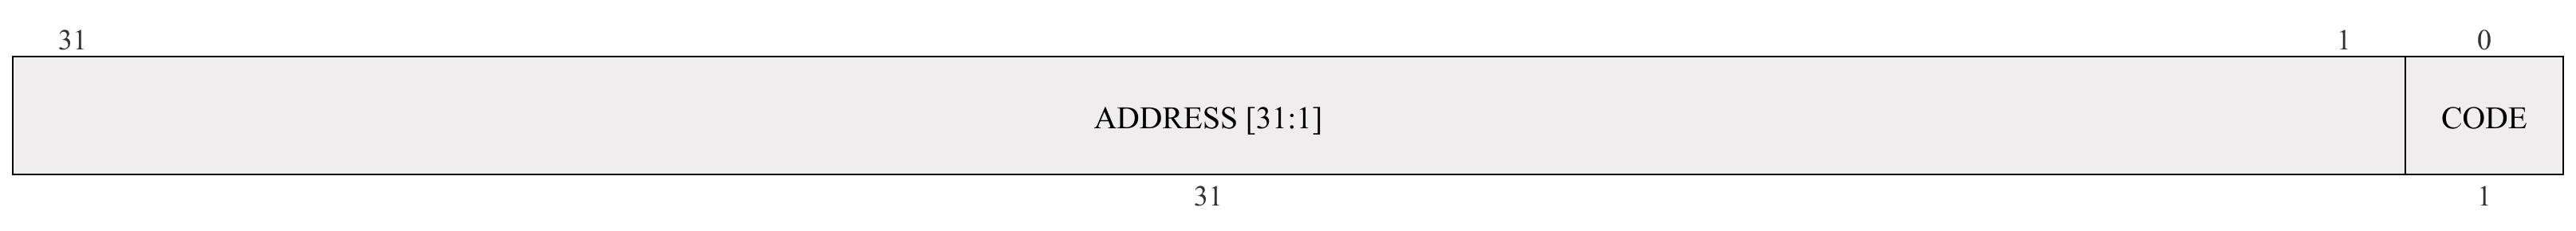
\includegraphics[width=.9\linewidth]{images/ecall_code.png}
  \caption{Encoding of register a7 during ecall}
  \label{fig:ecall}
\end{figure}

Forward edge controls are performed thanks to the Control Flow Graph and are further
explained in section \ref{sec:project_cfg} while backward edge controls are performed
thanks to the Shadow Stack and are further explained in section \ref{sec:project_ss}.

\section{Shadow Stack}
\label{sec:project_ss}

The file \textit{shadow\_stack.c} holds the configuration for the Shadow Stack.
The development of the Shadow Stack took inspiration from the formally verified
idea proposed by Matthieu Baty, Guillaume Hiet, and Pierre Wilke in their
article \textit{Work in progress: A formally verified shadow stack for RISC-V} \cite{shadowstack}.

The Shadow Stack is implemented as a standard Last-in-first-out stack (LIFO).
This is because the last jump that is performed in a code will always be the
first to return. This allowed us to build an effective and fast data structure that
consumes a small amount of memory.

The Shadow Stack allows two operations, \textit{push} and \textit{pop}. \textit{Push}
is used when a direct or indirect jump is made. If such a jump is considered legal,
its return address is pushed into the Shadow Stack and stored for later. Instead,
\textit{pop}, is used when a return is made. An address is \textit{popped} from
the Shadow Stack and a match between the popped value and the current return
address is made to decide whether the return instruction is legal or not.

\section{Control Flow Graph (CFG)}
\label{sec:project_cfg}

The Control Flow Graph of the binary is extracted during the instrumentation phase.
As we have seen, if there are indirect jumps the script performs a simulation run
to retrieve source and destination addresses of each indirect jump. If there is
a simulation, the output is parsed to store the addresses in a list. After that,
the static extraction begins, in which we examine the dump file of the binary to
retrieve the source and destination addresses of each direct call. After all the
addresses have been gathered, the lists are ordered and injected in the file
\textit{cfg.c} which holds the configuration for the Control Flow Graph.

In this file, we can see the structure of the Control Flow Graph which is an
array where each position is occupied by a pair \textit{source-destination}.
Since the CFG will not change during execution we can define it statically and
provide no functions to add or remove elements. The only available function is \textit{check}
which asks for a pair of addresses as input and determines whether such a pair
is part of the CFG or not. The check is implemented using a binary search function
and the comparison is made using the function depicted in Figure \ref{fig:binsearch}.
With this function, the binary search first searches for the source address and,
only when found it searches for the destination address.

This implementation of the Control Flow Graph effectively reduces space
consumption to the bare minimum while providing a fast checking method ($\mathcal{O}
(\log{n})$). Another solution could be to use a Hash Table to store the addresses.
In this case, we would reduce the time required to access the CFG to $\mathcal{O}
(1)$. However, this works only with big enough Hash Tables, otherwise, we could face
many collisions, and the time required to find the correct entry would increase.
Still, this alternative solution could be perfect for situations in which we
care more about time than space.

\begin{figure}[htbp]
  \centering
  \begin{lstlisting}[style=CStyle]
int compare(const int* A, const int* B) {
  for (int i = 0; i < 2; ++i) {
    if (A[i] < B[i]) return -1;
    if (A[i] > B[i]) return 1;
  }
  return 0;
}
 \end{lstlisting}
  \caption{Comparison for binary search}
  \label{fig:binsearch}
\end{figure}

\section{Physical Memory Protection (PMP)}
\label{sec:project_pmp}

In this project, the role of the PMP is to protect the Shadow Stack and the Control
Flow Graph from unauthorized modifications. To ensure that both these data
structures are secured four memory regions have been created. Each region's configuration
can be seen in Table \ref{tab:pmpregions}

\begin{table}
  \centering
  \begin{tabular}{|c|c|c|c|}
    \hline
    \textbf{Region Start}           & \textbf{Region End}           & \textbf{Type} & \textbf{Privileges} \\
    \hline
    0x00000000                      & End of .sdata region          & TOR           & R-W                 \\
    \hline
    Start of interrupt vector table & End of interrupt vector table & TOR           & R-W-X               \\
    \hline
    Start of Shadow Stack           & End of Control Flow Graph     & TOR           & R-W                 \\
    \hline
    Start of main                   & 0x90000000                    & TOR           & R-W-X               \\
    \hline
  \end{tabular}
  \caption{PMP memory regions}
  \label{tab:pmpregions}
\end{table}

The first region covers all the space between 0x00000000 and the end of the .sdata
region with read and write privileges, since this region contains only static data
there is no need to allow execution.

The second region covers the interrupt vector table and its functions, since
this region is accessed only in Machine mode and we need to execute instructions
we need to provide read, write, and instruction execution privileges.

The third region is the one that covers both the Shadow Stack and the Control
Flow Graph. For this reason, we need to restrict privileges to read and write. We
can't set this region as read-only since we need to modify the Shadow Stack during
execution.

The last region covers all the addresses from the start of the main function up to
the end of the memory. This region also includes user code and, since we need to
execute the code, we need to configure this region with read, write, and
instruction execution privileges.

This PMP configuration effectively helps to prevent unauthorized modifications
to critical components such as the Shadow Stack and the Control Flow Graph. Thanks
to this, we are sure that whatever value we read from these data structures will
be safe and trustable.

\section{Forward and Backward Edge Controls}
\label{sec:project_controls}

The most critical part of this project is about validating jump and return instructions
and this is done inside the interrupt vector table.

Forward edge controls are made thanks to the Control Flow Graph while backward edge
controls are made thanks to the Shadow Stack.

In this section, each control will be carefully explained to show how they work
and why they provide a certain degree of security.

\subsection{Forward Edge Controls}
\label{subsec:forward}

To perform a forward edge control we need three things. The first is the source
address, the second is the destination address, and the third is an oracle that
tells us if the pair source-destination is valid. As already explained the destination
address is retrieved from \textit{a7} which is passed as the ecall code. The source
register instead can be retrieved from mepc \ref{subsec:mepc}. As we have seen, when
a trap is taken mepc holds the address of the instruction that was interrupted.
Since the ecall generates the trap we can just add $4$ (size of the ecall) to
the address stored in mepc to retrieve the source address. Now that we have the pair
of addresses to check we can use the Control Flow Graph as the oracle. As
already explained, the CFG is computed before compilation and is securely stored
in a safe memory region so we can consider it as a trusted oracle.

So, when we need to perform a forward edge control, we can just send the source and
destination addresses to the \textit{check} function of the CFG. Such function performs
a binary search inside the CFG to see whether that specific pair is part of the original
CFG. If the search succeeds the function returns a positive value and the jump
is considered legal while, if the search does not succeed the instruction is aborted
and the execution terminates to prevent any possible damage.

Whenever a forward edge control succeeds we know that the related jump instruction
will eventually return so we need to store its return address inside the Shadow Stack.
To do so, we need to retrieve the return address but, since a call will always
return to its next instruction, we can just compute $source \ address + 2$ (size
of \textit{jal} and \textit{jalr}) to retrieve it. After that, the address is pushed
into the Shadow Stack, and the execution is resumed with the interrupted jump
instruction.

\subsection{Backward Edge Controls}
\label{subsec:backward}

To perform a backward edge control we need two things. The first is the
destination address and the second is an oracle that tells us if such address is
valid. As we have seen, the destination address is retrieved from \textit{a7} which
is passed as the ecall code. In this case, the oracle is the Shadow Stack.

So, when we need to perform a backward edge control, we can just pop an address from
the Shadow Stack and match the destination address with the popped one. If the
addresses are the same we consider the return instruction legal while, if they are
different the execution is terminated.

Whenever a backward edge control succeeds we must do nothing since the value has
already been removed from the Shadow Stack and no other modifications are needed.
Thus, the execution is resumed with the interrupted return instruction.

\section{Proof of Concept (PoC)}
\label{sec:project_poc}

In this section, we will see why the proposed solution effectively provides security
capabilities to a non-trusted and insecure code. Figure \ref{fig:functioning}
depicts an abstraction of the project's flow.

\begin{figure}[htbp]
  \centering
  \def\stackalignment{r}\stackunder{ 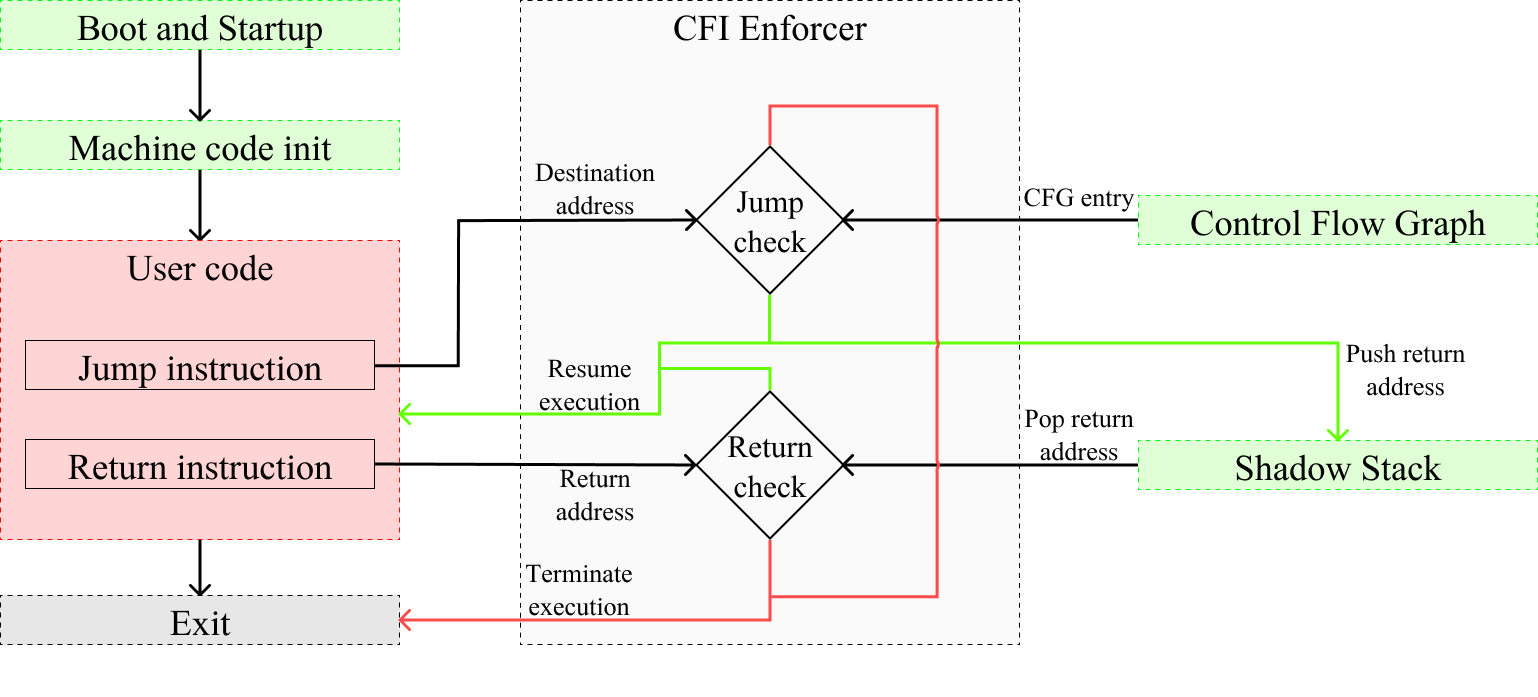
\includegraphics[width=.9\linewidth]{images/functioning.png} } %
  {\scriptsize }
  \caption{Abstraction of the flow of execution}
  \label{fig:functioning}
\end{figure}

We have already seen that the \textit{Boot and Startup} and \textit{Machine code
init} sections are used to configure the board and the machine configuration respectively.
This part of the code is trusted so we are sure the machine will be configured
properly. The only way to corrupt this part of the execution would be to modify the
source code before compilation but, this is out of the project's scope.

The same is true for the \textit{CFI Enforcer} section which is responsible for managing
edge controls as well as other interrupts and exceptions. Even in this case, the
source code has to be modified to tamper with the security features.

On the other hand, the \textit{User code} section is untrusted and we can't make
any assumptions on its functioning. The code could be well-written and somewhat
secure but it could be full of flaws and we must prevent any attack that could
be perpetrated through it. To do so, we use forward and backward edge controls
together with the Shadow Stack and the Control Flow Graph.

As already said, the Shadow Stack and the CFG are the most critical points of the
project. We must secure them since they serve as oracles and we must be able to
trust the data they contain. Since the CFG is configured statically we are sure that
it can't be modified during execution, the Shadow Stack instead is designed to
change since we need to push and pop values from it. However, since we protected
the Shadow Stack with the PMP we can be sure that only privileged code has
access to it and any other access generates a trap that is handled through the
interrupt vector table. This means that, even if one tries to add or remove
values from the stack the operation will be aborted immediately and our trust in
the Shadow Stack remains intact.

Now we will go through every possible scenario that could happen during a normal
execution.

As soon as a forward edge control is requested we check that the pair source-destination
is valid thanks to the CFG. Let's say that an attacker tampered with the code to
perform an unauthorized jump, in this case, the CFG will not contain such a pair
since we said that it can't be modified. In this case, the unauthorized jump is detected
and the code terminates immediately. Instead, if the pair is legal according to the
CFG the jump is considered safe and the return address is pushed into the Shadow
Stack. Note that since we compute the return address each time instead of
trusting the one provided by the user code we are sure that the value inserted
in the stack is correct and we can trust it.

If a backward edge control is requested instead, we check that the return address
provided by the user code is the one we are expecting by popping the last value that
was inserted in the Shadow Stack. Again, let's say that an attacker tampered with
the code to perform an unauthorized return, in this case, the addresses will not
match and the execution is terminated. Note that the fact that we can trust the
Shadow Stack is highly dependent on the configuration of the PMP. This is because,
without a proper configuration, it would be possible for an attacker to push a value
into the Shadow Stack and then tamper with the return address to effectively return
to an unauthorized address.

Moreover, when we try to push a value into a full Shadow Stack the execution is
terminated. This is needed because if we are not able to push the address into the
Shadow Stack we will not be able to make the next backward edge control and thus,
the security would be compromised. Note that the same happens when we try to pop
a value from an empty Shadow Stack since this means that we are checking a return
instruction that was never meant to be performed.

Lastly, we could design the enforcement of the backward edge controls in another
way. If we need to control a return address and there is a mismatch we could force
the user code to return to the address stored in the Shadow Stack which we know is
safe. While this solution enforces Control Flow Integrity securely we can't be
sure that the stack (referring to the normal stack used to store registers) has
not been compromised and thus, terminating execution is a much safer choice.

So, we have seen that this project effectively enforces Control Flow Integrity
on an untrusted user application and that its security functionalities work as
expected to prevent any attempt to perform unauthorized operations.
